% !TEX program = lualatex
% Compile from 2026/week12; figures are generated by make_figures.py.
\documentclass[12pt,aspectratio=43]{beamer}
% Shared Beamer design. Load after \documentclass using \input.
% Engine: LuaLaTeX. Fonts: UD Digi Kyokasho N (regular/bold), Arial.
\usepackage{luatexja-fontspec}
\setmainjfont[BoldFont={UD Digi Kyokasho N Bold}]{UD Digi Kyokasho N}
\setsansjfont[BoldFont={UD Digi Kyokasho N Bold}]{UD Digi Kyokasho N}
\setmonojfont[BoldFont={UD Digi Kyokasho N Bold}]{UD Digi Kyokasho N}
% Liberation Sans keeps the layout usable on systems without Arial.
\IfFontExistsTF{Arial}{
  \setmainfont{Arial}
  \setsansfont{Arial}
  \setmonofont{Arial}
}{
  \setmainfont{Liberation Sans}
  \setsansfont{Liberation Sans}
  \setmonofont{Liberation Sans}
}
\renewcommand{\kanjifamilydefault}{\gtdefault}

% Typeset mathematics with a dedicated TeX math font, independent of Arial.
\usefonttheme{professionalfonts}
\usepackage[mathrm=sym]{unicode-math}
\setmathfont{Latin Modern Math}
\setoperatorfont{\symup}

\definecolor{courseblue}{HTML}{4472C4}
\definecolor{ruleblue}{HTML}{8FAADC}
\setbeamercolor{normal text}{fg=black,bg=white}
\setbeamercolor{structure}{fg=courseblue}
\setbeamercolor{frametitle}{fg=black,bg=white}
\setbeamercolor{title banner}{fg=white,bg=courseblue}
\setbeamerfont{frametitle}{size=\fontsize{18}{22}\selectfont,series=\mdseries}
\setbeamerfont{quote}{shape=\upshape}
\setbeamersize{text margin left=9mm,text margin right=9mm}
\setbeamertemplate{navigation symbols}{}
\setbeamercolor{page number}{fg=gray,bg=white}
\setbeamertemplate{footline}{%
  \begin{beamercolorbox}[wd=\paperwidth,ht=2.5mm,dp=1.5mm]{page number}
    \hfill{\fontsize{8}{9}\selectfont
      \ifnum\value{framenumber}>0
        \insertframenumber\,/\,\inserttotalframenumber
      \fi}\hspace*{3mm}
  \end{beamercolorbox}}
\setbeamertemplate{headline}{%
  \hfill\textcolor{gray}{\fontsize{6}{7}\selectfont
    \hypersetup{linkcolor=gray}% Keep Beamer's title links in the header color.
    \ifnum\value{framenumber}=0 \insertshortdate\enspace\fi
    \insertshorttitle\space\insertshortsubtitle}\hspace{2mm}\vspace{1.5mm}}
\setbeamertemplate{frametitle}{%
  \vspace{2mm}\centering\insertframetitle\par
  \vspace{-1mm}{\color{ruleblue}\rule{.44\paperwidth}{.5pt}}\par
  \vspace{2mm}}
\setbeamercolor{itemize item}{fg=courseblue}
\setbeamercolor{itemize subitem}{fg=black}
\setbeamercolor{itemize subsubitem}{fg=black}
\setbeamertemplate{itemize item}{\textbullet}
\setbeamertemplate{itemize subitem}{\textnormal{-}}
\setbeamertemplate{itemize subsubitem}{\textnormal{-}}
\setlength{\parskip}{.45em}
\hypersetup{colorlinks=true,urlcolor=courseblue}

% Use \titlepage inside a [t,noframenumbering] frame. The background extends
% 1 mm past both page edges to avoid hairline gaps in PDF viewers.
\setbeamertemplate{title page}{%
  \vspace{2mm}
  \begin{beamercolorbox}[wd=\paperwidth,ht=43mm,dp=13mm,colsep*=1mm,center]{title banner}
    {\fontsize{32}{40}\selectfont\inserttitle\par}
    \vspace{2mm}
    {\fontsize{20}{24}\selectfont\insertsubtitle\par}
  \end{beamercolorbox}
  \vspace{10mm}
  \hfill\insertauthor
}

\graphicspath{{figures/}}
\usepackage{listings}
\usepackage{upquote}
\IfFontExistsTF{Consolas}{\newfontfamily\codefont{Consolas}}{\newfontfamily\codefont{Liberation Mono}}
\definecolor{codevalue}{HTML}{7A3E9D}
\definecolor{codebuiltin}{HTML}{006DB0}
\definecolor{codestring}{HTML}{267348}
\newcommand{\code}[1]{{\codefont #1}}
\lstdefinestyle{python}{
  language=Python,
  basicstyle=\codefont\fontsize{12}{14}\selectfont,
  keywordstyle=\color{codebuiltin},
  stringstyle=\color{codestring},
  showstringspaces=false,
  columns=fullflexible,
  keepspaces=true,
  upquote=true,
  tabsize=4,
  breaklines=false,
  backgroundcolor=\color{black!4},
  frame=single,framerule=0pt,framesep=1.7mm,
  xleftmargin=1.7mm,xrightmargin=1.7mm,
  aboveskip=1mm,belowskip=0.5mm,
  literate=*{0}{{{\color{codevalue}0}}}1
    {1}{{{\color{codevalue}1}}}1 {2}{{{\color{codevalue}2}}}1
    {3}{{{\color{codevalue}3}}}1 {4}{{{\color{codevalue}4}}}1
    {5}{{{\color{codevalue}5}}}1 {6}{{{\color{codevalue}6}}}1
    {7}{{{\color{codevalue}7}}}1 {8}{{{\color{codevalue}8}}}1
    {9}{{{\color{codevalue}9}}}1
}
\lstset{style=python}
\setbeamercolor{lesson note}{fg=black,bg=courseblue!9}
\newenvironment{lessonbox}
  {\begin{beamercolorbox}[wd=\linewidth,sep=1.5mm]{lesson note}}
  {\end{beamercolorbox}\par}

\title{計算物理学B}
\subtitle{第十二回：偏微分方程式1}
\author{野垣 康介、藤本 悠輝}
\date{2027/1/19}
\hypersetup{pdftitle={計算物理学B 第十二回：偏微分方程式1},pdfauthor={野垣 康介、藤本 悠輝}}

\begin{document}

\begin{frame}[t,noframenumbering]
  \titlepage
\end{frame}

\begin{frame}{講義予定}
  \setlength{\parskip}{0pt}
  2026年度 第2学期（火曜3限）
  \par\vspace{2mm}
  \begingroup\centering
    \renewcommand{\arraystretch}{1.05}
    \begin{tabular}{@{}l@{\hspace{2mm}}l@{\hspace{4mm}}l@{\hspace{2mm}}l@{}}
      10/6 & 四則演算 & 12/8 & モンテカルロ1 \\
      10/27 & 制御文（for, if） & 12/15 & モンテカルロ2 \\
      11/6（金） & 関数 & 12/22 & 微分方程式1 \\
      11/10 & 配列（NumPy） & 1/12 & 微分方程式2 \\
      11/17 & 可視化（matplotlib） & 1/19 & \textcolor{courseblue}{\textbf{偏微分方程式1}} \\
      11/24 & 数値微分 & 1/26 & 偏微分方程式2 \\
      12/1 & 数値積分 & 2/2 & 根の探索 \\
      \multicolumn{2}{c}{\small 〜中間レポート〜} &
      \multicolumn{2}{c}{\small 〜期末レポート〜}
    \end{tabular}\par
  \endgroup
  \vspace{2mm}
  {\small \textcolor{courseblue}{10/20は出張で休講。} 11/6（金）は火曜授業の振替。\par}
\end{frame}

\begin{frame}{授業で使うリンク}
  \begin{itemize}
    \setlength{\itemsep}{3mm}
    \item Google Colab：{\small\url{https://colab.research.google.com/?hl=ja}}
    \item 講義資料（GitHub）：{\small\url{https://github.com/nogaki/Computational_Physics_B}}
    \item 今週のノートブック：\code{2026/week12/week12.ipynb}
    \item 今週のPDF：\code{2026/week12/slide.pdf}
  \end{itemize}
  \vfill
  {\footnotesize 日付・休講日は2026年度の講義予定に基づく。}
\end{frame}

\begin{frame}[t]{GitHubからColabへ}
  \begin{enumerate}
    \setlength{\itemsep}{4mm}
    \item GitHubで\code{2026/week12/week12.ipynb}を開き、URLをコピーする。
    \item Colabの「ファイル」→「ノートブックを開く」→「GitHub」を選ぶ。
    \item URLを貼り付けて検索し、ノートブックを開く。
  \end{enumerate}
  \vspace{3mm}
  \begin{lessonbox}
    \textbf{「ドライブにコピーを保存」を実行する}\par
    \small 開いただけでは自分のGoogle Driveに保存されない。編集前にコピーを作る。
  \end{lessonbox}
\end{frame}

\begin{frame}[t]{今回の内容：偏微分方程式}
  \begin{itemize}
    \setlength{\itemsep}{3mm}
    \item 境界値問題：ラプラス方程式と反復法
    \item 初期値問題：熱方程式の有限差分
    \item FTCS法の安定性とvon Neumann解析
    \item 陰解法・Crank--Nicolson法との比較
    \item 実習では1次元波動方程式を解く
  \end{itemize}
  \vfill
  \begin{lessonbox}
    今回は差分式を自分で実装する。配列計算にはNumPy、三重対角方程式にはSciPyを使う。
  \end{lessonbox}
\end{frame}

\begin{frame}[t]{偏微分方程式が記述するもの}
  \small
  \begin{itemize}
    \setlength{\itemsep}{3mm}
    \item 静電ポテンシャル：\(\nabla^2\phi=-\rho/\epsilon_0\)
    \item 温度・密度の拡散：\(\partial_t u=D\nabla^2u\)
    \item 弦や音の変位：\(\partial_t^2u=c^2\nabla^2u\)
    \item 流体速度：Navier--Stokes方程式
  \end{itemize}
  \vspace{3mm}
  \begin{columns}[T,onlytextwidth]
    \begin{column}{.48\textwidth}
      \begin{block}{境界値問題}
        領域の境界で値を指定し、空間分布を求める。
      \end{block}
    \end{column}
    \begin{column}{.48\textwidth}
      \begin{block}{初期値問題}
        初期分布と境界条件から時間発展を求める。
      \end{block}
    \end{column}
  \end{columns}
\end{frame}

\begin{frame}[t]{有限差分法}
  格子点上の値を未知数とし、微分を近傍点の差で近似する。
  \[
    u'(x_i)\approx\frac{u_{i+1}-u_{i-1}}{2\Delta x},\qquad
    u''(x_i)\approx\frac{u_{i+1}-2u_i+u_{i-1}}{(\Delta x)^2}.
  \]
  \begin{itemize}
    \item 長方形格子の問題を小さなコードで実装できる。
    \item 複雑な形状には有限要素法・有限体積法などが向く。
    \item 精度は格子幅、時間刻み、境界条件の扱いに依存する。
  \end{itemize}
\end{frame}

\begin{frame}[t]{例：正方形領域のラプラス方程式}
  電荷のない領域では、静電ポテンシャルは
  \[
    \nabla^2\phi=0.
  \]
  上辺（角を除く）を\(V\)、ほかの辺を\(0\)に固定する。
  格子幅は\(a=L/M\)で、内部点のポテンシャルを求める。\par
  \vspace{1mm}
  \centering
  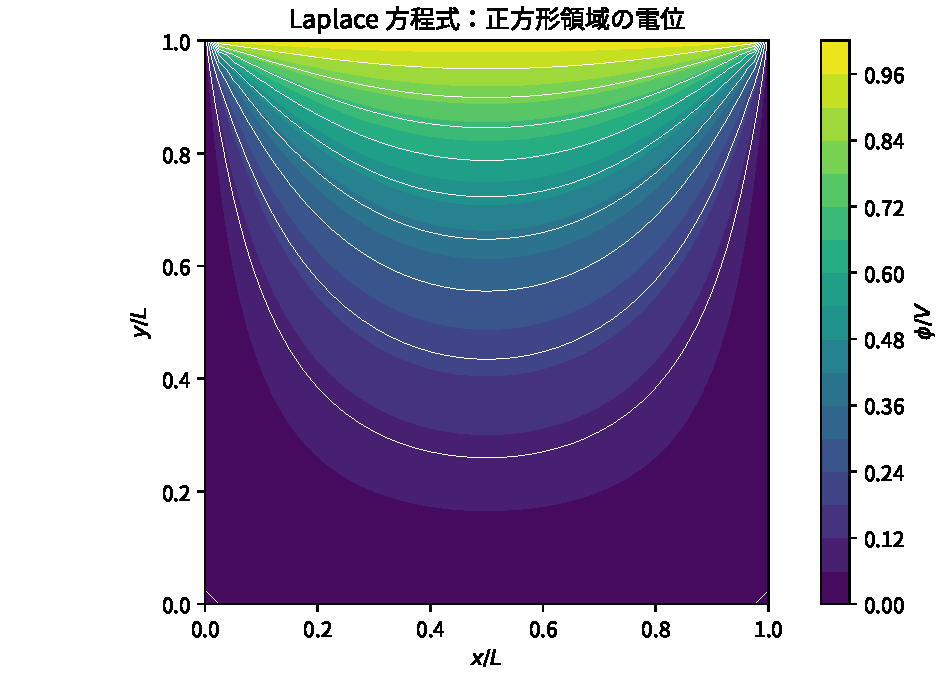
\includegraphics[width=.58\linewidth,height=36mm,keepaspectratio]{laplace_potential.pdf}
\end{frame}

\begin{frame}[t]{5点差分と境界条件}
  2階微分を中心差分で置き換えると、内部点で
  \[
    \phi_{i+1,j}+\phi_{i-1,j}+\phi_{i,j+1}+\phi_{i,j-1}-4\phi_{i,j}=0.
  \]
  よって各点の値は4近傍の平均になる。
  \[
    \phi_{i,j}=\frac{\phi_{i+1,j}+\phi_{i-1,j}+\phi_{i,j+1}+\phi_{i,j-1}}{4}.
  \]
  \begin{itemize}
    \item 境界値は反復中も変えない。
    \item 角の値は隣り合う辺の条件と整合するように置く。
  \end{itemize}
\end{frame}

\begin{frame}[t]{連立一次方程式に書き直す}
  内部格子点の数は\((M-1)^2\)。未知数を一つのベクトルに並べると
  \[
    A\boldsymbol{\phi}=\boldsymbol{b}.
  \]
  \begin{itemize}
    \item 行列\(A\)は疎行列で、各行の非零要素は最大5個。
    \item \(n=(M-1)^2\)個の未知数を密行列で直接解くと、計算量は概ね\(O(n^3)=O(M^6)\)。
    \item 疎行列法や反復法なら、構造を利用して大きな格子を扱いやすい。
  \end{itemize}
\end{frame}

\begin{frame}[t]{Jacobi法}
  \(n\)回目の格子全体から、次の格子全体を同時に作る。
  \[
    \phi^{(n+1)}_{i,j}=\frac{1}{4}\left(
    \phi^{(n)}_{i+1,j}+\phi^{(n)}_{i-1,j}
    +\phi^{(n)}_{i,j+1}+\phi^{(n)}_{i,j-1}\right).
  \]
  \begin{itemize}
    \item 更新前と更新後の2配列を使う。
    \item 境界条件は各反復で保持する。
    \item 反復差または残差が十分小さくなったら止める。
  \end{itemize}
\end{frame}

\begin{frame}[t]{Gauss--Seidel法}
  格子点を順番に更新し、すでに更新した近傍の値を次の点で使う。
  \[
    \phi^{(n+1)}_{i,j}=\frac{1}{4}\left(
    \phi^{(n)}_{i+1,j}+\phi^{(n+1)}_{i-1,j}
    +\phi^{(n)}_{i,j+1}+\phi^{(n+1)}_{i,j-1}\right).
  \]
  \begin{itemize}
    \item 多くの場合、Jacobi法より少ない反復で収束する。
    \item 更新順に依存するため、並列化しにくい。
    \item 更新差だけでなく、差分方程式の残差も確認する。
  \end{itemize}
\end{frame}

\begin{frame}[t]{SOR法：Gauss--Seidel更新を緩和する}
  通常の平均値を\(\bar\phi_{i,j}\)とすると、更新を
  \[
    \phi^{(n+1)}_{i,j}=\phi^{(n)}_{i,j}
    +\omega\left(\bar\phi_{i,j}-\phi^{(n)}_{i,j}\right)
  \]
  とする。
  \begin{itemize}
    \item \(\omega=1\)：Gauss--Seidel法。
    \item \(1<\omega<2\)：過緩和。反復回数を減らせる場合がある。
    \item 2次元ラプラス問題では\(0<\omega<2\)で収束する。
    \item 最適値は格子や問題に依存し、経験的に選ぶ。
  \end{itemize}
\end{frame}

\begin{frame}[t]{同じ境界値問題を3つの方法で解く}
  \begin{columns}[T,onlytextwidth]
    \begin{column}{.56\textwidth}
      \small
      \begin{itemize}
        \item Jacobi：全点を別配列に更新。
        \item Gauss--Seidel：更新済みの値を使う。
        \item SOR：更新幅を\(\omega\)倍する。
        \item 反復差は停止の目安。残差で方程式を満たすか確認する。
      \end{itemize}
    \end{column}
    \begin{column}{.42\textwidth}
      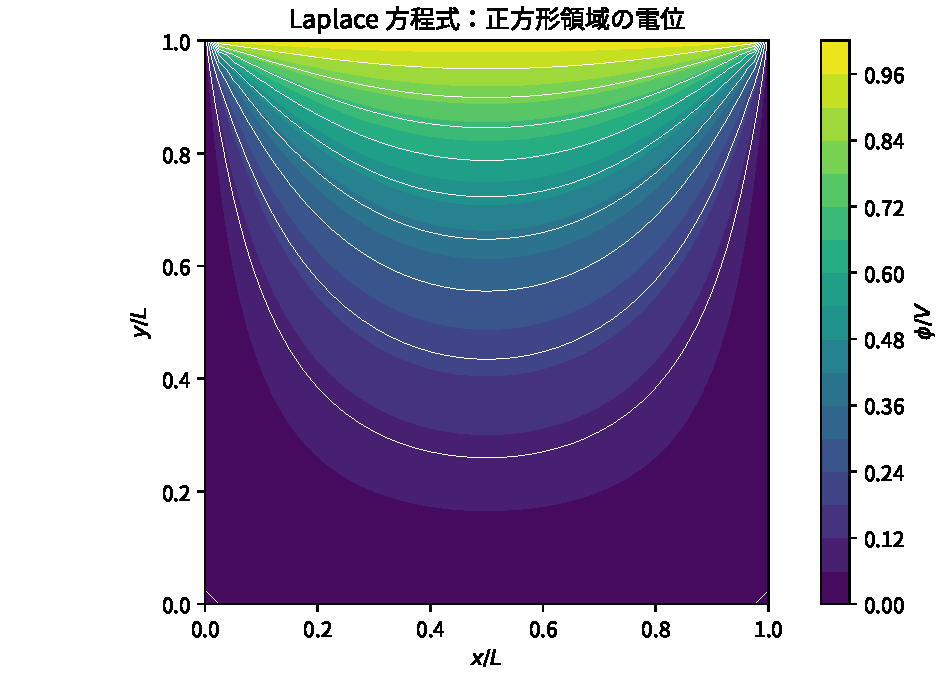
\includegraphics[width=\linewidth]{laplace_potential.pdf}
    \end{column}
  \end{columns}
  \vspace{2mm}
  \small 図は内部値0から始めたSOR解（\(\omega=1.75\)）。NotebookではJacobi法とSOR法の残差を比べる。
\end{frame}

\begin{frame}[t]{初期値問題：熱方程式}
  1次元の温度分布\(u(t,x)\)は、熱拡散率\(D\)を用いて
  \[
    \frac{\partial u}{\partial t}=D\frac{\partial^2u}{\partial x^2}
  \]
  に従う。
  \begin{itemize}
    \item 初期条件：\(u(0,x)=u_0(x)\)。
    \item 境界条件：\(u(t,0)=u_L\)、\(u(t,L)=u_R\)。
    \item 固定境界なら、時間がたつと定常分布へ近づく。
  \end{itemize}
  \small \(D\)の単位は\(\mathrm{m^2/s}\)。
\end{frame}

\begin{frame}[t,fragile]{FTCS法：時間を前進、空間を中心差分}
  \(\Delta t=h\)、\(\Delta x=a\)、\(r=Dh/a^2\)とおく。
  \[
    u^{n+1}_k=u^n_k+r\left(u^n_{k+1}-2u^n_k+u^n_{k-1}\right).
  \]
  次の時刻の値を現在時刻だけから計算する陽解法である。
  \begin{lstlisting}
for k in range(1, N):
    lap = u[k+1] - 2*u[k] + u[k-1]
    unew[k] = u[k] + r*lap
  \end{lstlisting}
  \small 両端の値は境界条件として別に設定する。
\end{frame}

\begin{frame}[t]{von Neumann安定性解析}
  1つの波数成分\(u_k^n=G^n e^{ik\theta}\)を差分式に代入する。
  \[
    G=1-4r\sin^2\!\left(\frac{\theta}{2}\right).
  \]
  全ての波数で\(|G|\leq1\)となる条件は
  \[
    0\leq r=\frac{D\Delta t}{(\Delta x)^2}\leq\frac12.
  \]
  \begin{itemize}
    \item 格子を細かくすると、安定な時間刻みは\((\Delta x)^2\)に比例して小さくなる。
    \item 安定条件を外れると、高波数成分が増幅する。
  \end{itemize}
\end{frame}

\begin{frame}[t]{FTCSの増幅率}
  \centering
  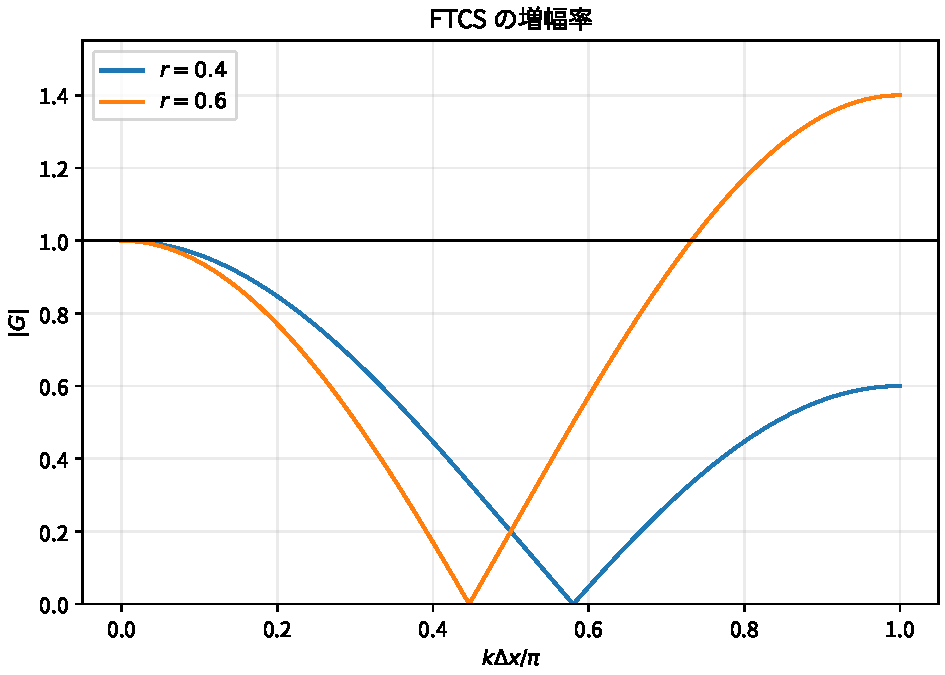
\includegraphics[width=.74\linewidth,height=43mm,keepaspectratio]{ftcs_stability.pdf}
  \par\vspace{2mm}
  \small \(r=0.4\)では全波数の\(|G|\leq1\)。\(r=0.6\)では格子間隔に近い高波数が増幅する。
\end{frame}

\begin{frame}[t]{温度分布の例：ステンレス棒}
  \begin{itemize}
    \setlength{\itemsep}{0.5mm}
    \item 長さ1 cm、熱拡散率\(D=4.25\times10^{-6}\,\mathrm{m^2/s}\)。
    \item 初期温度20 $^\circ$C、左端50 $^\circ$C、右端0 $^\circ$C。
  \end{itemize}
  \centering
  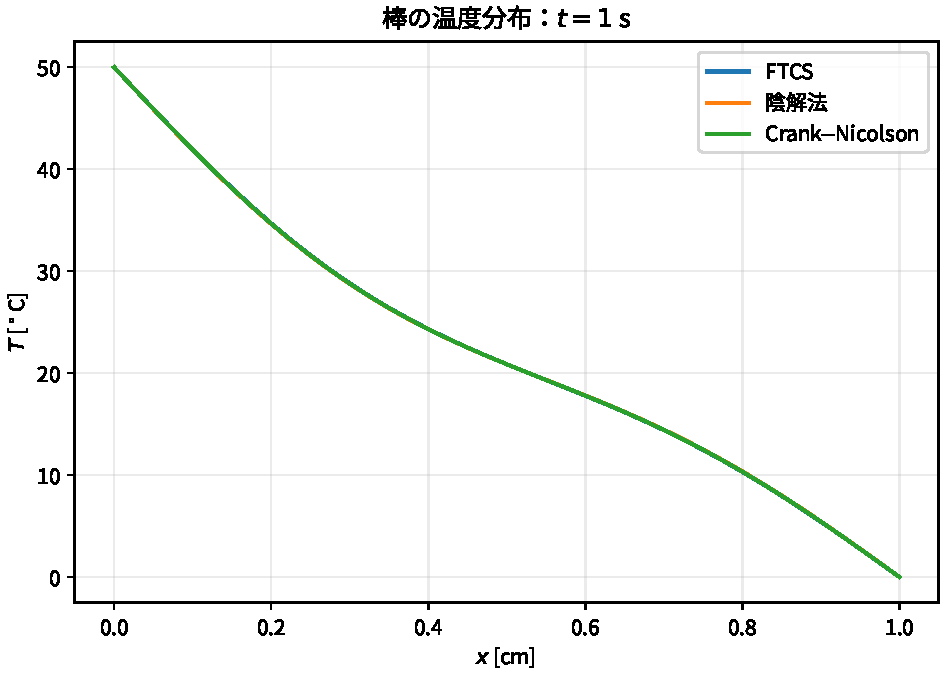
\includegraphics[width=.72\linewidth,height=39mm,keepaspectratio]{heat_methods.pdf}
  \par\small 40区間、\(r=0.4\)、\(t=1\) s。各線はFTCS・陰解法・Crank--Nicolson法。
\end{frame}

\begin{frame}[t,fragile]{陰解法}
  時間微分を後退差分で近似する。
  \[
    -r u^{n+1}_{k-1}+(1+2r)u^{n+1}_{k}-r u^{n+1}_{k+1}=u^n_k.
  \]
  \begin{itemize}
    \item 各時間ステップで三重対角方程式を解く。
    \item 熱方程式ではvon Neumann解析上、全ての\(r\geq0\)で安定。
    \item 大きな刻み幅では安定でも、時間変化を粗く表す。
  \end{itemize}
  \begin{lstlisting}
unew[1:N] = solve_banded((1, 1), ab, rhs)
  \end{lstlisting}
\end{frame}

\begin{frame}[t]{Crank--Nicolson法}
  前時刻と次時刻の空間微分を平均する。
  \[
    -\frac r2 u^{n+1}_{k-1}+(1+r)u^{n+1}_k-\frac r2 u^{n+1}_{k+1}
    =\frac r2u^n_{k-1}+(1-r)u^n_k+\frac r2u^n_{k+1}.
  \]
  \begin{itemize}
    \item 時間について2次精度。熱方程式では全ての\(r\geq0\)で安定。
    \item 陰解法と同様に三重対角方程式を解く。
    \item 大きな時間刻みでは安定性と単調性は別問題。
  \end{itemize}
\end{frame}

\begin{frame}[t]{差分法を選ぶときの確認事項}
  \begin{columns}[T,onlytextwidth]
    \begin{column}{.58\textwidth}
      \begin{itemize}
        \item 格子幅と時間刻みを記録する。
        \item 境界値を更新式に正しく加える。
        \item 安定条件を満たすか確認する。
        \item 格子や刻み幅を変え、解がどう変わるか比較する。
      \end{itemize}
    \end{column}
    \begin{column}{.39\textwidth}
      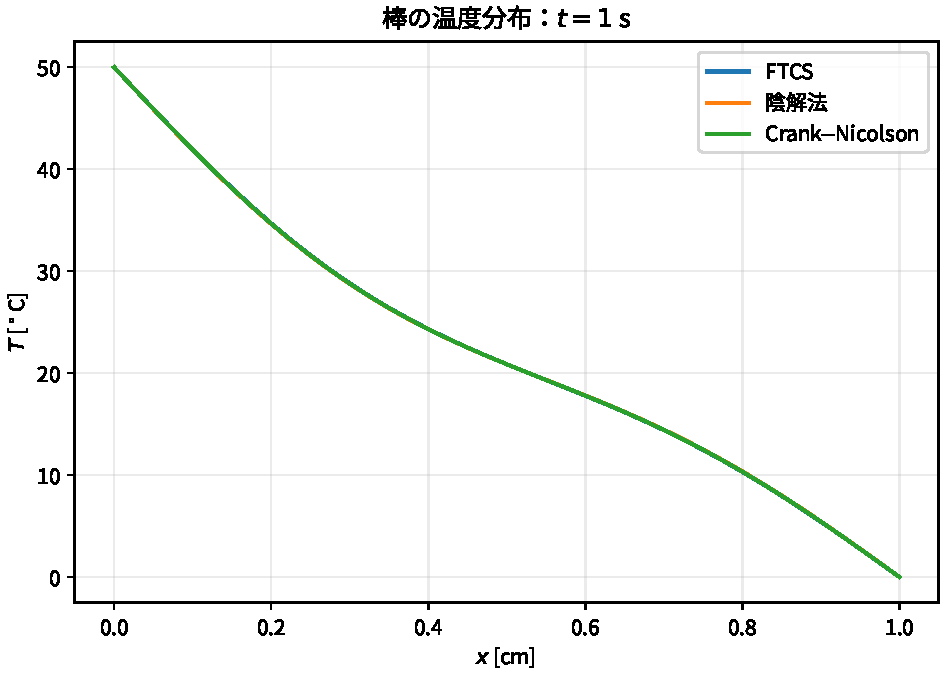
\includegraphics[width=\linewidth]{heat_methods.pdf}
    \end{column}
  \end{columns}
  \vspace{2mm}
  \begin{lessonbox}
    解が有限値でも正しいとは限らない。残差・境界条件・刻み幅依存性を確かめる。
  \end{lessonbox}
\end{frame}

\begin{frame}[t]{実習：波動方程式を解く}
  次の1次元波動方程式を考える。
  \[
    \frac{\partial^2\phi}{\partial t^2}
    =c^2\frac{\partial^2\phi}{\partial x^2}.
  \]
  \begin{itemize}
    \item \(\phi(0,x)\)と\(\partial_t\phi(0,x)\)を与える。
    \item 固定端の境界条件を設定する。
    \item Notebookの導出を参考に、Crank--Nicolson法を実装する。
    \item 指定時刻の変位を描き、刻み幅を変えて比較する。
  \end{itemize}
  \vfill
  \begin{lessonbox}
    \code{2026/week12/week12.ipynb}の最後のコードセルは実習用の空欄。
  \end{lessonbox}
\end{frame}

\begin{frame}[t]{まとめと参考}
  \begin{itemize}
    \item 空間微分を差分化すると、境界値問題は連立方程式になる。
    \item 熱方程式FTCS法の安定条件は\(D\Delta t/(\Delta x)^2\leq1/2\)。
    \item 陰解法・Crank--Nicolson法は各時刻で連立方程式を解く。
    \item 数値解では、安定性・境界条件・残差を確認する。
  \end{itemize}
  \vfill
  {\footnotesize
    野本拓也・是常隆・有田亮太郎『実践計算物理学』共立出版。\\
    M. Newman, \emph{Computational Physics}.\\
    \url{https://github.com/vlvovch/PHYS6350-ComputationalPhysics}}
\end{frame}

\end{document}
